\section{TADs \& leurs relations}
\subsection{Décomposition modulaire}

\bframes{
\small
5 modules (+ \texttt{main.c}) ont été créés pour la réalisation du TP\@:
\begin{enumerate}
    \item Le fichier \code{main.c} qui contient la fonction main qui permet de lancer le programme.\\
    
    \item Le module \code{inp.c}\\
    Définit la struct \code{struct Inp} qui stock et gère l'input entré par l'utilisateur, pour ensuite l'utiliser dans \code{lock.c}.

    \item Le module \code{lock.c}\\
    Utilise l'entrée de l'utilisateur pour ensuite remplir un \code{struct flock} avec les données nécessaires, et effectuer l'appel correspondant à \code{fcntl} pour lock/unlock les fichers.
\end{enumerate}
}



\bframes{
\begin{enumerate}
    \stepcounter{enumi} \stepcounter{enumi} \stepcounter{enumi}

    \item Le module \code{optprsr.c} (repris du TP02, openssl) \\
    contient 3 fonctions, servant à gérer les options passées en paramètres.\\
    \vspace{0.3cm}
    
    \item Le module \code{files.c} (repris du TP03, ultra-cp) \\
    S'occupe de la gestion fichers, (existence, type, taille etc.), des path des fichiers (absolute path, concatenation...) et de la gestion des erreurs liées à ces opérations.
    \vspace{0.3cm}

    \item Le module \code{util.c} (repris du TP03, ultra-cp) \\
      Fonctions servant divers usages allant de la gestion d'erreurs à la gestion de chaînes de caractères, en passant par des wrappers qui incluent lesdites fonctions de gestions d'erreurs.\\
            
    \end{enumerate}
}

%

\subsection{Structures de données utilisées}
  \begin{frame}[fragile]{\sn : \ssn}
     Une structure de donnée (opaque) \code{Inp} à été définie dont une explication brève a été donnée précédemment.
    Voici un apperçu de ses attributs:\\
    \lstinline{ //inp.c}\\
    \vspace{-0.05cm}
    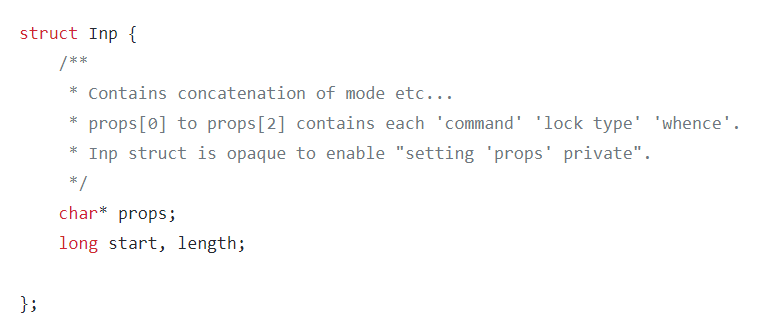
\includegraphics[scale=0.6]{images/inp-struct.png}\\

    \vspace{-0.3cm}
    \lstinline{ //inp.h}\\
    \vspace{-0.05cm}
    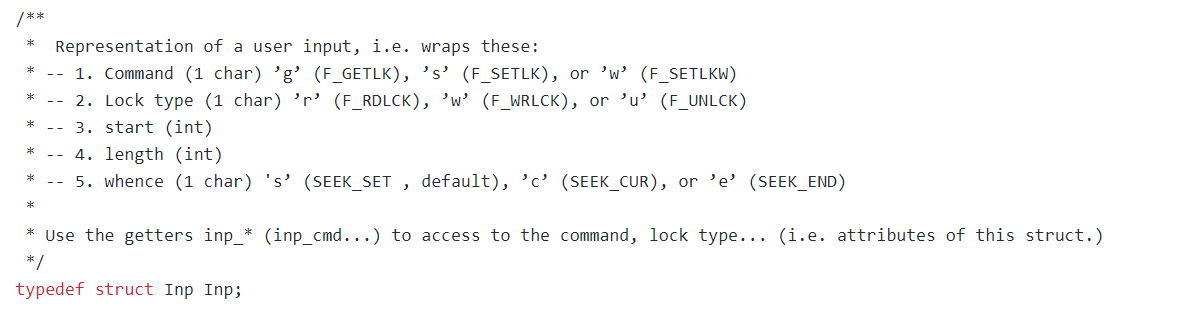
\includegraphics[scale=0.55]{images/inp-structh.png}
  \end{frame}


\begin{frame}[fragile]{\sn}
    
Avoir stocké toutes les options dans une seule chaîne de caractère et non pas plusieurs variables permet de l'initialiser comme suit :\\

\begin{lstlisting}
    int parseInput(char* cmd, char* ltype, long* start, long* length, char* whence) {
        /* ... */
        int an = sscanf(buf, "%s %s %ld %ld %s", cmd, ltype, start, length, whence);  // argument number
        switch (an) { /* ... */ }
    }
    Inp* inp = malloc(sizeof(Inp));
    inp->props = calloc(strArgNb + 1, sizeof(char)); // strArgNb = 3
    //...
    parseInput(&inp->props[0], &inp->props[1], &inp->start, &inp->length, &inp->props[2]);
    // ...

\end{lstlisting}

{\footnotesize 
 (Où \code{parseInput()} fait principalement un \code{fscanf} avec les arguments qui lui\\ sont passés puis vérifie la validité de chacun et gère les éventuelles erreurs)
}
\end{frame}


%
%
\subsection{Décomposition fonctionnelle}
\bframes{
\vspace{-0.5cm}
    Les principales fonctions utilisés sont simplements des fonction de parsing d'input, manipulations de struct, wrapper simplifiant l'utilisation de fonctions de librairie C $\, $ + gestion d'erreur\ldots \\
    
    Le \quo{réel} vérouillage de fichier\ldots$\ $ est réalisé par des appels \code{fcntl()}, du type
    \code{fcntln(fd, fl\_cmd, \&fl)}\\
    où \code{fl} est une \code{struct flock} qui a été converti directement depuis une \code{struct Inp} et \code{fl\_cmd} est la commande entrée par l'utilisateur stockée dans la \code{struct Inp}.

    \vspace{0.2cm}
    En effet, une très grande partie du code est de la gestion d'erreur et du parsing d'argument en entrée, (voir fonction \code{lock()} du module \code{lock}, 1 ligne d'appel à \code{fcntl} et $\approx$ 65 lignes d'analyse de code d'erreur retourné, en fonctions de tel ou tel command (\code{F\_GETLK}, \code{F\_SETLK}\ldots)\\
    
    La partie qui \quo{change} vraiment (outre la théorie sur les locks) est la mini structure de REPL / Shell que la CLI fournie par notre programme doit avoir.
    }
    
    \bframes{
    En résumé, les mécanismes de gestions d'erreurs et de parsing d'arguments étant un thème déjà longuement abordé dans les précédents et suivants TPs, ils ne seront pas plus détaillés ici.
    }
